\documentclass[11pt]{report}

\usepackage{epsf,amsmath,amsfonts}
\usepackage{graphicx}
\usepackage{longtable}
\usepackage{hyperref}
\usepackage{color}

\setlength{\topmargin}{0in}
\setlength{\headheight}{0in}
\setlength{\headsep}{0in}
\setlength{\textheight}{9.0in}
\setlength{\textwidth}{6.5in}
\setlength{\evensidemargin}{0in}
\setlength{\oddsidemargin}{0in}

\setlength\LTleft\parindent
\setlength\LTright\fill

\newcommand{\version}{1.0}


\newcommand{\core}{atmosphere}

\begin{document}

\title{MPAS -- Atmosphere Model User's Guide}

\author{Version \version}

\maketitle

\chapter*{Foreword}
\label{chap:foreword}

This user's guide describes the Model for Prediction Across Scales -- Atmosphere
(MPAS-A) Version \version. Updates to MPAS-A, including the most recent code,
user's guide, and test cases, may be found at \url{http://mpas-dev.github.com}.

MPAS-A is the non-hydrostatic atmosphere model built within a general MPAS
framework, which is being developed collaboratively between Los Alamos National
Laboratory (LANL) and the National Center for Atmospheric Research (NCAR).
Common functionality required by different MPAS models, such as parallel
input/output, time management, block decomposition, etc., is provided by the
MPAS framework, while development of specific model ``cores'' is handled by the
individual groups.

\vspace{8pt}
\noindent
{\bf Contributors to this guide:}\\
Michael Duda, Laura Fowler, Bill Skamarock, and Conrad Roesch\\
{\bf Additional contributors to the compilation chapter and appendices:}\\
Doug Jacobsen, Todd Ringler

\vspace{8pt}
\noindent
{\it The National Center for Atmospheric Research (NCAR) is operated by the
University Corporation for Atmospheric Research (UCAR) and is sponsored by the
National Science Foundation.  Any opinions, findings, conclusions, or
recommendations expressed in this publication are those of the authors and do
not necessarily reflect the views of the National Science Foundation.}


\tableofcontents

%--------------------------------------------------------------------------------------------
% MPAS-A Overview
%--------------------------------------------------------------------------------------------

\chapter{MPAS-A Overview}
\label{chap:atmosphere_overview}

The Model for Prediction Across Scales -- Atmosphere (MPAS-A) is a
non-hydrostatic atmosphere model that is part of a family of
Earth-system component models, collectively known as MPAS.  All MPAS
models have in common their use of centoidal Voronoi tessellations for
their horizontal meshes, which has motivated the development of a common
software framework that provides a high-level driver program and
infrastructure for providing parallel execution, input and output, and
other software infrastructure.

\section{Features}

Key features of MPAS-A include:

\begin{itemize}
\item Fully-compressible, non-hydrostatic dynamics
\item Split-explicit Runge-Kutta time integration
\item something,
\item something,
\item something.
\end{itemize}

At present, MPAS-A includes parameterizations of physical processes
taken from the Weather Research and Forecasting (WRF) Model
\footnote{\url{http://www.wrf-model.org/}.}. Specifically, MPAS-A has
support for:

\begin{itemize}
\item Radiation: CAM and RRTMG long-wave and short-wave radiation schemes
\item Land-surface: NOAH land-surface model
\item Surface-layer: Monin-Obukhov
\item Boundary-layer: YSU PBL scheme
\item Convection: Kain-Fritsch and Tiedtke convection parameterizations
\item Cloud microphysics: WSM6 and Kessler schemes
\end{itemize}

\section{Model components}

MPAS-A employs two main components: the model itself, which includes
atmospheric dynamics and physics; and an initialization component for
generating initial conditions and update files for sea-surface
temperature and sea ice. Both of these components are built as ``cores''
within the MPAS software framework and make use of the same driver
program and software infrastructure, but are compiled separately as
distinct executables. 

\begin{figure}[htb]
\begin{center}
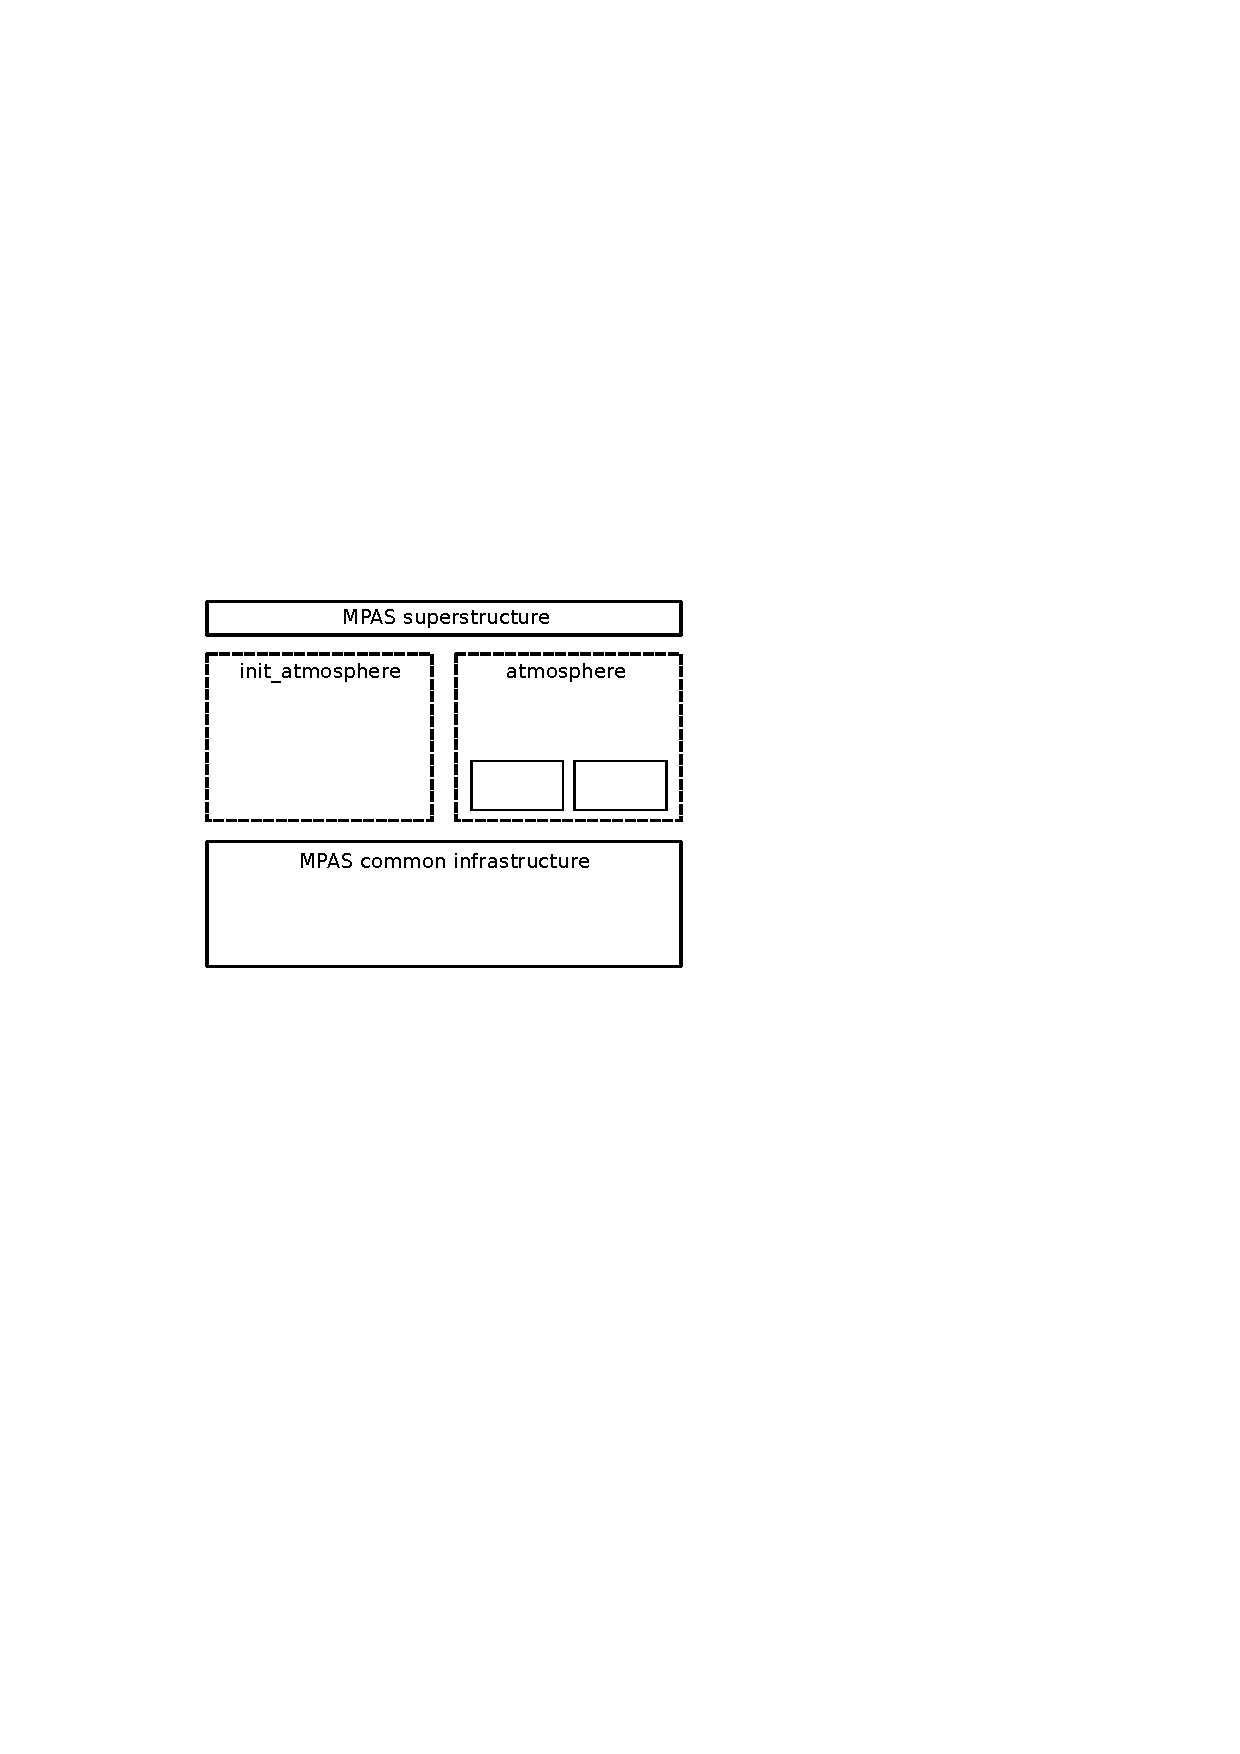
\includegraphics[width=3.5in]{atmosphere/figures/mpas-a_components.pdf}
\caption{Blah.}
\label{fig:atm_components}
\end{center}
\end{figure}

The details of compiling these components are given in Chapter
\ref{chap:mpas_build_instructions}, and the basic steps to create initial
conditions and run the MPAS-A model are outlined in Chapter
\ref{chap:running_mpas_a}.

\chapter{Building MPAS}
\label{chap:mpas_build_instructions}

\section{Prequisites}

To build MPAS, compatible C and Fortran compilers are required. Additionally,
the MPAS software relies on the PIO parallel I/O library to read and write model
fields, and the PIO library requires the standard netCDF library as well as the
parallel-netCDF library from Argonne National Labs. All libraries must be
compiled with the same compilers that will be used to build MPAS. Section
\ref{sec:build_io} summarizes the basic procedure of installing the required I/O
libraries for MPAS.

In order for the MPAS makefiles to find the PIO, parallel-netCDF, and netCDF
include files and libraries, the environment variables {\tt PIO}, {\tt PNETCDF},
and {\tt NETCDF} should be set to the root installation directories of the PIO,
parallel-netCDF, and netCDF installations, respectively. 

An MPI installation such as MPICH or OpenMPI is also required, and there is no
option to build a serial version of the MPAS executables. There is currently no
support for shared-memory parallelism with OpenMP within the MPAS framework.


\section{Compiling I/O Libraries}
\label{sec:build_io}

{\bf IMPORTANT NOTE:} {\em The instructions provided in this section for
installing libraries have been successfully used by MPAS developers, but due to
differences in library versions, compilers, and system configurations, it is
recommended that users consult documentation provided by individual library
vendors should problems arise during installation. The MPAS developers take no
responsibility for third-party libraries.} \vspace{12pt}

Although most recent versions of the I/O libraries should work, the most tested
versions of these libraries are: netCDF 4.1.3, parallel-netCDF 1.3.1, and PIO
1.6.7. The netCDF and parallel-netCDF libraries must be installed before
building PIO library.

\subsection{netCDF}

Version 4.1.3 of the netCDF library may be downloaded from
\url{http://www.unidata.ucar.edu/downloads/netcdf/netcdf-4\_1\_3/index.jsp}.
Assuming the gfortran and gcc compilers will be used, the following shell
commands are generally sufficient to install netCDF.

\vspace{12pt}
{\tt > setenv FC gfortran}

{\tt > setenv F77 gfortran} 

{\tt > setenv F90 gfortran}

{\tt > setenv CC gcc} 

{\tt > ./configure --prefix=XXXXX --disable-dap --disable-netcdf-4 --disable-cxx \hfill\break --disable-shared --enable-fortran} 

{\tt > make all check}

{\tt > make install}
\vspace{12pt}

Here, {\tt XXXXX} should be replaced with the directory that will serve as the
root installation directory for netCDF.  {\em Before proceeding to compile PIO
the {\tt NETCDF\_PATH} environment variable should be set to the netCDF root
installation directory.}

Certain compilers require addition flags in the CPPFLAGS environment variable.
Please refer to the netCDF installation instructions for these flags.

\subsection{parallel-netCDF}

Version 1.3.1 of the parallel-netCDF library may be downloaded from
\url{https://trac.mcs.anl.gov/projects/parallel-netcdf/wiki/Download}.  Assuming
the gfortran and gcc compilers will be used, the following shell commands are
generally sufficient to install parallel-netCDF.

\vspace{12pt}
{\tt > setenv MPIF90 mpif90}

{\tt > setenv MPIF77 mpif90} 

{\tt > setenv MPICC mpicc}  

{\tt > ./configure --prefix=XXXXX} 

{\tt > make}

{\tt > make install}
\vspace{12pt}

Here, {\tt XXXXX} should be replaced with the directory that will serve as the
root installation directory for parallel-netCDF.  {\em Before proceeding to
compile PIO the {\tt PNETCDF\_PATH} environment variable should be set to the
parallel-netCDF root installation directory.}


\subsection{PIO}

Due to the rapid development pace of the PIO library, it is recommended to
obtain and install PIO following the instructions at
\url{http://www.cesm.ucar.edu/models/pio/} for building PIO.

After PIO is built and installed the {\tt PIO} enviroment variable should be set to 
the directory where PIO was installed. Recent versions of PIO support a {\tt --prefix}
option, which specifies the installation directory, while older versions do not,
in which case the {\tt PIO} environment variable should be set to the directory where
PIO was compiled.

\section{Compiling MPAS}

{\bf IMPORTANT NOTE:} {\em Before compiling MPAS, the {\tt NETCDF}, {\tt
PNETCDF}, and {\tt PIO} environment variables must be set to the library
installation directories as described in the previous section.} \vspace{12pt}

The MPAS code uses only the `make' utility for compilation. Rather than
employing a separate configuration step before building the code, all
information about compilers, compiler flags, etc., is contained in the top-level
{\tt Makefile}; each supported combination of compilers (i.e., a configuration)
is included in the {\tt Makefile} as a separate make target, and the user
selects among these configurations by running {\tt make} with the name of a
build target specified on the command-line, e.g.,

\vspace{12pt}
{\tt > make gfortran}
\vspace{12pt}

\noindent to build the code using the GNU Fortran and C compilers. Some of the
available targets are listed in the table below, and additional targets can be
added by simply editing the {\tt Makefile} in the top-level directory.

\vspace{12pt}
\begin{longtable}{| l | l | l | l |}
\hline
Target & Fortran compiler & C compiler & MPI wrappers \\ \hline \hline
{\tt xlf} & xlf90 & xlc & mpxlf90 / mpcc \\ \hline
{\tt pgi} & pgf90 & pgcc & mpif90 / mpicc \\ \hline
{\tt ifort} & ifort & gcc & mpif90 / mpicc \\ \hline
{\tt gfortran} & gfortran & gcc & mpif90 / mpicc \\ \hline
{\tt g95} & g95 & gcc & mpif90 / mpicc \\ \hline
\end{longtable}
\vspace{12pt}

The MPAS framework supports multiple {\em cores} --- currently a shallow water
model, an ocean model, a non-hydrostatic atmosphere model, and a non-hydrostatic
atmosphere initialization core --- so the build process must be told which core
to build. This is done by either setting the environment variable {\tt CORE} to
the name of the model core to build, or by specifying the core to be built
explicitly on the command-line when running {\tt make}. For the atmosphere
core, for example, one may run either

\vspace{12pt}
{\tt > setenv CORE atmosphere}

{\tt > make gfortran}
\vspace{12pt}

\noindent or

\vspace{12pt}
{\tt > make gfortran CORE=atmosphere}
\vspace{12pt}

If the {\tt CORE} environment variable is set and a core is specified on the
command-line, the command-line value takes precedence; if no core is specified,
either on the command line or via the {\tt CORE} environment variable, the build
process will stop with an error message stating such.  Assuming compilation is
successful, the model executable, named {\tt \$\{CORE\}\_model} (e.g., {\tt
sw\_model}), should be created in the top-level MPAS directory.

In order to get a list of available cores, one can simply run the top-level {\tt
Makefile} without setting the {\tt CORE} environment variable, or passing the
core via the command-line. An example of the output from this can be seen
below.

{\small
\begin{verbatim}
> make
( make error )

Usage: make target CORE=[core] [options]

Example targets:
    ifort
    gfortran
    xlf
    pgi

Availabe Cores:
    atmos_physics
    atmosphere
    init_atmosphere
    ocean
    sw

Available Options:
    DEBUG=true    - builds debug version. Default is optimized version.
    USE_PAPI=true - builds version using PAPI for timers. Default is off.
    TAU=true      - builds version using TAU hooks for profiling. Default is off.
    AUTOCLEAN=true    - forces a clean of infrastructure prior to build new core.

Ensure that NETCDF, PNETCDF, PIO, and PAPI (if USE_PAPI=true) are environment variables
that point to the absolute paths for the libraries.

************ ERROR ************
No CORE specified. Quitting.
************ ERROR ************
\end{verbatim}
}

\section{Cleaning}

To remove all files  that were created when the model was built,
including the model executable itself, {\tt make} may be run for the
`clean' target:

\vspace{12pt}
{\tt > make clean}
\vspace{12pt}

As with compiling, the core to be cleaned is specified by the {\tt CORE}
environment variable, or by specifying a core explicitly on the
command-line with {\tt CORE=}.

\chapter{Preparing meshes}
\label{chap:mpas_grid_preparation}

This chapter describes the steps used to prepare SCVT meshes for use in MPAS-A.
For quasi-uniform meshes, very little preparation is actually needed, and
generally, one only needs to prepare mesh decomposition files --- files that
describe the decomposition of the SCVT mesh across processors --- when running
MPAS-A using multiple MPI tasks. The procedure for creating these mesh
decomposition files is described in the first section. 

For variable-resolution SCVT meshes, the area of mesh refinement may be rotated
to any part of the sphere using a program, grid\_rotate, described in the second
section. This utility program may be obtained from the MPAS-A download page.
\section{Graph partitioning with METIS} 
\label{sec:metis}

Before MPAS can be run in parallel, a mesh decomposition file with an
appropriate number of partitions (equal to the number of MPI tasks that will be
used) is required. A limited number of mesh decomposition files, named {\tt
graph.info.part.*}, are provided with each mesh, as is the mesh
connectivity file, named {\tt graph.info}. In order to create new mesh
decomposition files for some particular number of MPI tasks, only the {\tt
graph.info} file is required.  The currently supported method for partitioning
a graph.info file uses the METIS software
(http://glaros.dtc.umn.edu/gkhome/views/metis).  The serial graph partitioning
program, METIS (rather than ParMETIS or hMETIS) should be sufficient for
quickly partitioning any mesh usable by MPAS.

After installing METIS, a {\tt graph.info} file may be partitioned into $N$
partitions by running

\vspace{12pt}
{\tt > gpmetis graph.info} $N$
\vspace{12pt}

\noindent The resulting file, {\tt graph.info.part.}$N$, can then be copied into
the MPAS run directory before running the model with $N$ MPI tasks.


\section{Relocating refinement regions on the sphere}
\label{sec:grid_rotate} 

The purpose of the grid\_rotate program is simply to rotate an MPAS mesh file,
moving a refinement region from one geographic location to another, so that the
mesh can be re-used for different applications. This utility was developed out
of the need to save computational resources, since generating an SCVT ---
particularly one with a large number of generating points or a high degree of
refinement --- can take considerable time.

To build the grid\_rotate program, the Makefile should first be edited to set
the Fortran compiler to be used; if the netCDF installation pointed to by the
{\tt NETCDF} environment variable was build with a separate Fortran interface
library, it will also be necessary to add {\tt -lnetcdff} just before {\tt
-lnetcdf} in the Makefile. After editing the Makefile, running `make' should
result in a grid\_rotate executable file.

Besides the MPAS grid file to be rotated, grid\_rotate requires a namelist file,
{\tt namelist.input}, which specifies the rotation to be applied to the mesh.
The namelist variables are summarized in the table below
   
\vspace{12pt}
\begin{longtable}{|p{3.25in} |p{2.5in}|}
\hline
config\_original\_latitude\_degrees & original latitude of any point on the sphere \\ \hline
config\_original\_longitude\_degrees & original longitude of any point on the sphere \\ \hline
config\_new\_latitude\_degrees &  latitude to which the original point should be shifted \\ \hline
config\_new\_longitude\_degrees &  longitude to which the original point should be shifted \\ \hline
config\_birdseye\_rotation\_counter\_clockwise\_degrees & rotation about a vector from the sphere center through the original point \\ \hline
\end{longtable}
\vspace{12pt}

\noindent Essentially, one chooses any point on the sphere, decides where that
point should be shifted to, and specifies any change to the orientation (i.e.,
rotation) of the mesh about that point. 

Having set the rotation parameters in the {\tt namelist.input} file, the
grid\_rotate program should be run with two command-line options specifying the
original grid file name and the name of the rotated grid file to be produced,
e.g.,

\vspace{12pt}
{\tt > grid\_rotate grid.nc grid\_SE\_Asia\_refinement.nc}
\vspace{12pt}

The original grid file will not be altered, and a new, rotated grid file will be
created. The NCL script {\tt mesh.ncl} may be used to plot either of the
original or rotated grid files after suitable setting the name of the grid file
in the script.
   

%--------------------------------------------------------------------------------------------
% Running the MPAS non-hydrostatic atmosphere model
%--------------------------------------------------------------------------------------------

\chapter{Running the MPAS non-hydrostatic atmosphere model}
\label{chap:running_mpas_a}

\setlength\LTleft{0.0in}

Given an SCVT mesh, this chapter describes the two main steps to running the non-hydrostatic model: creating initial conditions and running the model itself.  This chapter makes use of two MPAS cores, {\tt init\_atmosphere} and {\tt atmosphere}, which are, respectively, used for initializing and running the non-hydrostatic atmospheric model.  Sections 3.1 and 3.2 of this chapter describe the creation of idealized and real-data non-hydrostatic initial condition files using the {\tt init\_atmosphere} core.   Section 3.3 describes the basic procedure of running the model itself.

Each section of this chapter follows a familiar pattern of compiling and executing MPAS model components, albeit using different cores depending on its intended use.  The compilation will create either an initialization or a model executable, which are named, respectively, {\tt init\_atmosphere\_model} and {\tt atmosphere\_model}.  In general, if an MPAS executable was compiled for serial use, simply call the executable by name. If compiled to be run in parallel, the executable is called with {\tt mpiexec} or {\tt mpirun}, for example:

\vspace{12pt}
{\tt > mpiexec -n 8 atmosphere\_model}
\vspace{12pt}


\noindent where {\tt 8} is the number of MPI tasks to be used.  In any case where {\tt n} $>$ 1, there must exist a corresponding graph decomposition file, e.g., {\tt graph.info.part.8}. For more on graph decomposition, see \S 2.4.  

\section{Creating idealized ICs}

There are several idealized test cases supported within the {\tt init\_atmosphere} model initialization core:

1 --- Jablonowski and Williamson baroclinic wave, no initial perturbation
\footnote{Jablonowski, C. and D.L. Williamson, 2006, A baroclinic instability test case for atmospheric model dynamical cores, {\em QJRMS}, 132, 2943-2975. doi:10.1256/qj.06.12.}

2 --- Jablonowski and Williamson baroclinic wave, with initial perturbation

3 --- Jablonowski and Williamson baroclinic wave, with normal-mode perturbation

4 --- squall line

5 --- super-cell

6 --- mountain wave\\
\\
Creating idealized initial conditions is fairly straightforward, as no external data are required and the starting date/time is irrelevant to building the {\tt init.nc} file that will be used to run the model.

The following steps summarize the creation of {\tt init.nc}:

\begin{itemize}
\item Include a {\tt grid.nc} file, which contains the SCVT mesh, in the working directory (\S 2)
\item If running in parallel, include a {\tt graph.info.part.*} file in the working directory (\S 2.4)
\item Compile MPAS with the {\tt init\_atmosphere} core specified (\S 1.2)
\item Create an appropriate {\tt namelist.input} configuration file (described below)
\item Run {\tt init\_atmosphere\_model} to create {\tt init.nc}
\end{itemize}~\\

Included in the MPAS directory is a sample initialization namelist, {\tt namelist.input.init\_atmosphere}, which can be copied or linked to the {\tt namelist.input} file for use in this step.  A number of the namelist parameters found in {\tt namelist.input.init\_atmosphere} are irrelevant to creating idealized conditions and can be removed or ignored.  The following table outlines the namelist parameters that are required; comments are given on the right for certain key parameters, and formal explanations for all namelist parameters can be found in Appendix A.


\begin{longtable}{p{3in}|p{3.25in}}

\&nhyd\_model\\
   config\_init\_case       = 1                      & a number between 1 and 6 corresponding to the cases listed at the beginning of this section\\
   config\_theta\_adv\_order = 3                     & advection order for theta \\
/\\
\\
\&dimensions\\
   config\_nvertlevels     = 41                      & the number of vertical levels to be used in the model \\
/\\
\\
\&io\\
   config\_input\_name         = 'grid.nc'           & the name of the netCDF grid file from \S2 \\
   config\_output\_name        = 'init.nc'           & the name of the IC file to be created \\
/\\
\\
\&decomposition\\
   config\_block\_decomp\_file\_prefix = 'graph.info.part.' & if running in parallel, needs to match the grid decomposition file prefix \\
/\\

\end{longtable}



\section{Creating real-data ICs}

Creating real-data initial conditions is similar to that of the idealized case described in the previous section, but is more involved as it requires interpolation of static geographic data (e.g., topography, land cover, soil category, etc.), surface fields such as SST, and the atmospheric initial conditions associated with a particular date/time.  The static datasets are the same as those used by the WRF model, and the surface fields and atmospheric initial conditions can be obtained from GFS data using the WRF pre-processing system (WPS).

Creating real-data initial conditions requires a single compilation of the {\tt init\_atmosphere} core, but the actual generation of the IC files will take place using three separate runs of {\tt init\_atmosphere}, where each of these runs is described individually in the following sub-sections.  While it is possible to condense the three real-data initialization steps into fewer executions, running each step separately will both improve clarity and, as will become apparent, save a significant amount of time when generating subsequent initial conditions, that is, when making initial conditions using the same mesh but different starting times.

The first of the three steps, described in \S 3.2.1, is the interpolation of static fields onto the mesh to create a {\tt static.nc} file.  This step cannot be run in parallel and takes considerably longer than the steps that follow, however, the fields being static, this step need only be run once for a particular mesh, regardless of the number of initial condition files that are ultimately created from the {\tt static.nc} output file.  Described in \S 3.2.2 is an optional step that creates a file {\tt surface.nc} that contains surface data at regular intervals. This file is used in the case where the model run makes periodic external updates to surface fields (currently only sea-ice and SST).  Finally, \S 3.2.3 describes the processing of the atmospheric initial conditions beginning with the {\tt static.nc} file created in \S 3.2.1.  Naturally, each of the initialization runs described in the three following sections will make use of a {\tt namelist.input} file, and as was the case for idealized initial conditions, the file {\tt namelist.input.init\_atmosphere} in the MPAS directory can be used as a starting point.  Not every variable in this namelist is needed for any particular step, and therefore each section will elaborate only on the namelist variables that are immediately relevant.

\subsection{Static fields}

The generation of a file {\tt static.nc} requires a set of static geographic data.  A suitable dataset can be obtained from the WRF model's download page \\
 \url{http://www.mmm.ucar.edu/wrf/users/download/get\_source.html}.  These static data files should be downloaded to a directory, which will be specified the {\tt namelist.input} file (described below) prior to running this interpolation step.  The result of this run will be the creation of a netCDF file ({\tt static.nc}), which is used in the two steps, described in \S 3.2.2 and \S 3.2.3, following this to create surface update files and dynamic initial conditions.  Note that {\tt static.nc} can be generated once and then used repeatedly to generate surface update and initial condition files for different start times.

The following steps summarize the creation of {\tt static.nc}:

\begin{itemize}
\item Download geographic data from the WRF download page (described above) 
\item Compile MPAS with the {\tt init\_atmosphere} core specified (\S 1.2)
\item Include a {\tt grid.nc} file in the working directory (\S 2)
\item Create an appropriate {\tt namelist.input} configuration file (described below)
\item Run {\tt init\_atmosphere\_model} {\em either in serial or with only one MPI task specified} to create {\tt static.nc}
\end{itemize}~\\
Note that it is critical for this step that the initialization core is run serially; if the core was compiled in parallel, one only MPI task must be used ({\tt mpiexec -n 1 init\_atmosphere\_model}).  The steps described in \S 3.2.2 and \S 3.2.3 may be run in serial or parallel.

\begin{longtable}{p{3.0in} |p{3.25in}}

\&nhyd\_model\\
   config\_init\_case       = 7                      & must be 7, the real-data initialization case \\
/\\
\\
\&dimensions                                         & the following two variables must be present now, though their values do not become significant until \S 3.2.3 \\
   config\_nvertlevels     = 41                      &  \\
   config\_nsoillevels     = 4                       &  \\
/\\
\\
\&data\_sources\\
   config\_geog\_data\_path  = '/WPS\_GEOG/'         & absolute path to static files obtained from the WRF download page\\
/\\
\\
\&preproc\_stages                                    & only the static\_interp stage should be enabled \\
   config\_static\_interp   = .true.                 & \\
   config\_vertical\_grid   = .false.                & \\
   config\_met\_interp      = .false.                & \\
   config\_input\_sst       = .false.                & \\
/\\
\\
\&io\\
   config\_input\_name         = 'grid.nc'           & the name of the netCDF grid file from \S 2 \\
   config\_output\_name        = 'static.nc'         & file name for static netCDF output \\
/\\

\end{longtable}


\subsection{Surface field updates}

This step is optional --- it is required only if surface fields are to be periodically updated during the model run.  The surface data could originate from any number of sources, though the most straightforward way to obtain a dataset in the appropriate format is to process GRIB data (e.g., GFS GRIB data) with the {\em ungrib} program of the WRF model's pre-processing system (WPS).  Detailed instructions for building and running the WPS, and the process of generating intermediate data files from GFS data, can be found in Chapter 3 of the WRF User Guide: \url{http://www.mmm.ucar.edu/wrf/users/docs/user\_guide/users\_guide\_chap3.htm}.

The following steps summarize the creation of {\tt surface.nc}:

\begin{itemize}
\item Include surface data intermediate files in the working directory
\item Include a {\tt static.nc} file in the working directory (\S 3.2.1)
\item If running in parallel, include a {\tt graph.info.part.*} in the working directory (\S 2.4)
\item Create an appropriate {\tt namelist.input} configuration file (see below)
\item Run {\tt init\_atmosphere\_model} to create {\tt surface.nc}
\end{itemize}


\begin{longtable}{p{3.0in} |p{3.25in}}

\&nhyd\_model\\
   config\_init\_case       = 8                      & must be 8, the surface field initialization case \\
   config\_start\_time      = '2010-10-23\_00:00:00' & time to begin processing surface data \\
   config\_stop\_time       = '2010-10-24\_00:00:00' & time to end processing surface data \\
/\\
\\
\&data\_sources\\
   config\_sfc\_prefix      = 'SST'                  & the prefix of the intermediate data files containing SST and sea-ice \\
   config\_fg\_interval     = 21600                  & interval between intermediate files to use for SST and sea-ice \\
/\\
\\
\\
\&preproc\_stages                                    & only the config\_input\_sst step should be enabled \\
   config\_static\_interp   = .false.                & \\
   config\_vertical\_grid   = .false.                & \\
   config\_met\_interp      = .false.                & \\
   config\_input\_sst       = .true.                 & \\
/\\
\\
\&io\\
   config\_input\_name          = 'static.nc'        & name of the netCDF static data file \S 3.2.1 \\
   config\_sfc\_update\_name    = 'surface.nc'       & surface-update file name \\
/\\
\\
\&decomposition\\
   config\_block\_decomp\_file\_prefix = 'graph.info.part.' & if running in parallel, needs to match the grid decomposition file prefix \\
/\\

\end{longtable}



\subsection{Vertical grid generation and initial field interpolation}

The final step for creating a real-data initial conditions file ({\tt init.nc}) is to generate a vertical grid, the parameters of which will be specified in the {\tt namelist.input} file, and to obtain an initial conditions dataset and interpolate it onto the model grid. As stated previously, while initial conditions could ultimately be obtained from many different data sources, here we assume the use of intermediate data files obtained from GFS data using the WPS ungrib program.  Detailed instructions for building and running the WPS, and how to generate intermediate data files from GFS data, can be found in Chapter 3 of the WRF user guide: \\
\url{http://www.mmm.ucar.edu/wrf/users/docs/user\_guide/users\_guide\_chap3.htm}.

The following steps summarize the creation of {\tt init.nc}:

\begin{itemize}
\item Include a WPS intermediate data file in the working directory
\item Include the {\tt static.nc} file in the working directory (\S 3.2.1)
\item If running in parallel, include a {\tt graph.info.part.*} file in the working directory (\S 2.4)
\item Create an appropriate {\tt namelist.input} configuration file (described below)
\item Run {\tt init\_atmosphere\_model} to create {\tt init.nc}
\end{itemize}


\begin{longtable}{p{3.0in} |p{3.25in}}

\&nhyd\_model\\
   config\_init\_case       = 7                      & must be 7 \\
   config\_theta\_adv\_order = 3                     & advection order for theta \\
   config\_start\_time      = '2010-10-23\_00:00:00' & time to process first-guess data \\
/\\
\\
\&dimensions\\
   config\_nvertlevels     = 41                      & number of vertical levels to be used in MPAS \\
   config\_nsoillevels     = 4                       & number of soil layers to be used in MPAS \\
   config\_nfglevels       = 38                      & number of vertical levels in intermediate file \\
   config\_nfgsoillevels   = 4                       & number of soil layers in intermediate file \\
/\\
\\
\&data\_sources\\
   config\_met\_prefix      = 'FILE'                 & the prefix of the intermediate file to be used for initial conditions \\
/\\
\\
\&vertical\_grid\\
   config\_ztop            = 30000.0                 & model top height (m) \\
   config\_nsmterrain      = 2                       & number of smoothing passes for terrain \\
   config\_smooth\_surfaces = .false.                 & whether to smooth zeta surfaces \\
/\\
\\
\&preproc\_stages                                    & \\
   config\_static\_interp   = .false.                & \\
   config\_vertical\_grid   = .true.                 & only these three stages should be enabled \\
   config\_met\_interp      = .true.                 & \\
   config\_input\_sst       = .false.                & \\
/\\
\\
\&io\\
   config\_input\_name         = 'static.nc'         & the netCDF static file \S 3.2.1 \\
   config\_output\_name        = 'init.nc'           & name of the IC file to be created \\
/\\
\\
\&decomposition\\
   config\_block\_decomp\_file\_prefix = 'graph.info.part.' & if running in parallel, needs to match the grid decomposition file prefix \\
/\\
\end{longtable}


\section{Running the model}

With the files {\tt init.nc} and, optionally, {\tt surface.nc}, generated as in the previous sections, we have completed the prerequisites to run the model.  The only step remaining before running the model itself is the configuration of {\tt namelist.input}.  As a starting point, the MPAS directory contains {\tt namelist.input.atmosphere}, along with three other namelists corresponding to the various idealized cases, that can be copied or linked to {\tt namelist.input}.  This section will discuss both running the model from a cold start and restarting the model from some point in a previous run.

The following steps summarize running the model:

\begin{itemize}
\item Include an initial condition netCDF file (e.g., {\tt init.nc}) in the working directory(\S 3.1, \S 3.2)
\item If using surface updates, include a surface netCDF file (e.g., {\tt surface.nc}) in the working directory (\S 3.2.2)
\item If running in parallel, include a graph decomposition file in the working directory (\S 2.4)
\item If the MPAS directory has not been cleaned since running initialization, run {\tt make clean} with the {\tt init\_atmosphere} core specified
\item Compile MPAS with the {\tt atmosphere} core specified (\S 1.2)
\item Create an appropriate {\tt namelist.input} configuration file (described below)
\item Run the compiled executable
\end{itemize}

Below is a list of variables in {\tt namelist.input} that pertain to input, output, and model restarts.  A number of namelist variables are not listed here (specifications for dynamical core configuration, physics parameters, etc.) and Appendix A should be consulted for the purpose and acceptable values of these parameters.

\begin{longtable}{p{3.0in} |p{3.25in}}

\&nhyd\_model                                        & \\
   config\_dt = 450.0                                & the model timestep; an appropriate value must be chosen relative to the grid cell spacing \\
   config\_start\_time = '2010-10-23\_00:00:00'      & the model start time corresponding to {\tt init.nc}\\
   config\_run\_duration = '5\_00:00:00'             & the duration of the model run; for format rules, see Appendix A \\
   config\_sfc\_update\_interval = 'none'            & the frequency of surface updates; for format rules, see Appendix A \\
/                                                    & \\
   config\_stop\_time  = '0000-01-16\_00:00:00'      & this can be used in place of {\tt config\_run\_duration} \\
                                                     & \\
\&io                                                 & \\
   config\_input\_name = 'init.nc'                   & the IC file from \S 3.1 or 3.2 \\
   config\_output\_name = 'output.nc'                & the name of the output netCDF file (if necessary, date/time will be inserted automatically) \\
   config\_restart\_name = 'restart.nc'              & the name given to restart files will that will be created (date/time will be inserted automatically) \\
   config\_output\_interval = '1\_00:00:00'          & the interval to write data to the output file\\
   config\_frames\_per\_outfile = 1                  & a non-negative integer; 0 specifies a single output file \\
   config\_sfc\_update\_name = 'surface.nc'          & only needed if using surface updates (file from \S 3.2.2) \\
/ 
\\
\&decomposition                                            & \\
   config\_block\_decomp\_file\_prefix = 'graph.info.part.' & if running in parallel, must match the prefix of the graph decomposition file \\
/                                                    & \\
\\
\&restart                                            & \\
   config\_restart\_interval = '1\_00:00:00'         & the interval to create restart files; for format rules, see Appendix A \\
   config\_do\_restart = .false.                     & if true, will select the appropriate {\tt restart.nc} file generated from a previous run \\
/ 
\end{longtable}

When running the model from a cold start, {\tt config\_start\_time} should match the time that was used when creating {\tt init.nc}, and the file names specified in the {\tt \&io} section should be present in the working directory.  The model output can be written to a single file, e.g., {\tt output.nc}, or written to multiple files differentiated by the date of the file's first output frame.  This behaviour is determined by the variable {\tt config\_frames\_per\_outfile}: if set to 0, all output will be written to the single file {\tt output.nc}, and any number greater than 0 determines the maximum number of output frames written per output file.  For example, given the namelist values displayed above, an output file would be written for each day of the model run and each file would contain a single output frame.  Dates are inserted automatically into the output file names, so the output would be {\tt output.2010-10-23\_00:00:00.nc, output.2010-10-24\_00:00:00.nc}, etc.  In this example, if {\tt config\_frames\_per\_outfile} were changed to 3, a new output file would be created every third day and each would contain three frames per file.

During the course of a model run, restart files are created at an interval specified by the namelist variable {\tt config\_restart\_interval}.  A unique restart file is created for each restart time, and as was the case when multiple output files are created, they are differentiated by the automatic insertion of the restart date in the filename.  For example, the namelist values listed above would create the files {\tt restart.2010-10-24\_00:00:00.nc, restart.2010-10-25\_00:00:00.nc}, etc. Unlike with history output files, no restart file is created at the model initial time.

Running the model from a restart file is similar to running the model from {\tt init.nc}.  The required changes are that {\tt config\_do\_restart} must be set to {\tt .true.} and {\tt config\_start\_time} must correspond to a restart file existing in the working directory.


%--------------------------------------------------------------------------------------------
% Plotting model output
%--------------------------------------------------------------------------------------------

\chapter{Visualization}
\label{chap:atmosphere_visualization}

Since the MPAS input and output files are in netCDF format, a wide variety of software
tools may be used to manipulate and visualize fields in these files. As a starting point, several NCL \footnote{NCAR Command Language; \url{http://ncl.ucar.edu}}
scripts are provided in the {\tt graphics/ncl} sub-directory
of the main MPAS directory for making the basic types of plots illustrated in Figure \ref{fig:ncl_plots}. Each of
these scripts reads the name of the file from which fields should be plotted from the environment variable {\tt FNAME},
and all but the mesh-plotting script read the time frame to be plotted from the environment variable {\tt T}. To plot
a field from the first frame (indexed from 0) of the file {\tt output.2010-10-23\_00:00:00.nc}, for example, one would set the 
following environment variables 

\vspace{12pt}
{\tt > setenv FNAME output.2010-10-23\_00:00:00.nc}

{\tt > setenv T 0}
\vspace{12pt}

\noindent before running one of the scripts. In general, the specific field to be plotted from the netCDF file must be set 
within a script before running that script. 

\begin{figure}[htb]
\begin{center}
\includegraphics[width=6.5in]{atmosphere/figures/ncl_plots.pdf}
\caption{Various plot types that can be produced from MPAS input or output files using example scripts provided with the MPAS code.
(a) A plot of an MPAS SCVT mesh against a filled map background. (b) A simple horizontal contour plot. (c) A cell-filled horizontal plot, with
individual cells of the mesh drawn as polygons colored according to the field value. (d) A vertical cross-section in height, with areas below the
terrain left unshaded.}
\label{fig:ncl_plots}
\end{center}
\end{figure}


\section{Meshes}

A plot showing just an MPAS SCVT mesh can be produced using the {\tt atm\_mesh.ncl} script, as in Figure \ref{fig:ncl_plots}(a). This script
reads a subset of the mesh description fields in Chapter \ref{chap:grid_information} and uses this information to draw the SCVT mesh over a 
color-filled map background. Parameters in the script can be used to control the type of map projection (e.g., orthographic, cylindrical equidistant, etc.), 
the colors used to fill land and water points, and the widths of lines used for the Voronoi cells.


\section{Horizontal contour plots}

Contour plots of horizontal fields can be produced with the {\tt atm\_contours.ncl} script, as in Figure \ref{fig:ncl_plots}(b). The particular
field to be plotted is set in the script and can in principle be drawn on any horizontal surface (e.g., a constant pressure
surface, a constant height surface, sea-level, etc.) if suitable vertical interpolation code is added to the script. Not shown in the figure are horizontal
wind vectors, which can also be added to the plot using example code provided in the script.


\section{Horizontal cell-filled plots}

For visualizing horizontal fields on their native SCVT grid, the {\tt atm\_cells.ncl} script may be used to produce horizontal cell-filled plots, 
as in Figure \ref{fig:ncl_plots}(c). This script draws each MPAS grid cell as a polygon colored according to the value of the field in that
cell; the color scale is automatically chosen based on the range of the field and the default NCL color table, though other color tables can
be selected instead.


\section{Vertical cross-sections}

Vertical cross-sections of fields can be created using the {\tt atm\_xsec.ncl} script, as in Figure \ref{fig:ncl_plots}(d). Before running this script,
a starting point and an ending point for the cross section must be given as latitude-longitude pairs near the top of the script, and the number of points along
the cross section should be specified. The script evenly distributes the specified number of points along the shortest great-circle arc from the 
starting point to the ending point, and for each point, the script uses values from the grid cell containing that point (i.e., a nearest-neighbor interpolation
to the horizontal cross-section points is performed); no vertical interpolation is performed, and the thicknesses and vertical heights of cells are
all drawn according to the MPAS vertical grid.




\input{atmosphere/mpas_atm_field_description.tex}
\input{atmosphere/mpas_atm_init_namelist_options.tex}
\input{atmosphere/mpas_atm_namelist_options.tex}

\appendix
\input{shared/mpas_grid_description.tex}
\chapter{Grid Information}
\label{chap:grid_information}

This chapter describes several of the MPAS grid variables and dimensions. The majority of these are common across all cores.

\section{Grid dimensions}

{\small
\begin{longtable}{|p{1.75in} |p{4.5in}|}
 \hline
        Time     &   netCDF record (unlimited) dimension \\ \hline
        nCells       &   Number of cells in the grid \\ \hline
        nEdges      &   Number of edges (cell faces) in the grid \\ \hline
        nVertices    &   Number of vertices (cell corners) in the grid \\ \hline
        nVertLevels     &   Number of vertical layers \\ \hline
        nVertLevelsP1   &   Number of vertical levels (nVertLevels + 1) \\ \hline
        maxEdges        &   Maximum number of neighbor cells of any cell \\ \hline
        maxEdges2       &   Twice maxEdges \\ \hline
        TWO              &   Constant value 2 \\ \hline
        THREE            &   Constant value 3 \\ \hline
        vertexDegree     &   Number of edges incident with each vertex (3 for Delaunay dual grid) \\ \hline
        FIFTEEN         &   Constant value 15 \\ \hline
        TWENTYONE       &   Constant value 21 \\ \hline
        R3               &   Constant value 3 \\ \hline
        StrLen          &   Length of strings \\ \hline
\end{longtable}
}

\section{Horizontal mesh fields}
\label{sec:mesh_fields}

{\small
\begin{longtable}{|p{2.75in} |p{3.5in}|}
 \hline
        double latCell(nCells)       & Cell center latitude (rad) \\ \hline
        double lonCell(nCells)       & Cell center longitude (rad) \\ \hline
        double xCell(nCells)         & Cell center x-coordinate (m, w.r.t. unit sphere) \\ \hline
        double yCell(nCells)         & Cell center y-coordinate (m, w.r.t. unit sphere) \\ \hline
        double zCell(nCells)         & Cell center z-coordinate (m, w.r.t. unit sphere) \\ \hline
        int indexToCellID(nCells)    & Global cell ID \\ \hline
        double latEdge(nEdges)       & Edge latitude (rad) \\ \hline
        double lonEdge(nEdges)       & Edge longitude (rad) \\ \hline
        double xEdge(nEdges)         & Edge x-coordinate (m, w.r.t. unit sphere) \\ \hline
        double yEdge(nEdges)         & Edge y-coordinate (m, w.r.t. unit sphere) \\ \hline
        double zEdge(nEdges)         & Edge z-coordinate (m, w.r.t. unit sphere) \\ \hline
        int indexToEdgeID(nEdges)    & Global edge ID \\ \hline
        double latVertex(nVertices)      & Vertex latitude (rad) \\ \hline
        double lonVertex(nVertices)      & Vertex longitude (rad) \\ \hline
        double xVertex(nVertices)        & Vertex x-coordinate (m, w.r.t. unit sphere) \\ \hline
        double yVertex(nVertices)        & Vertex y-coordinate (m, w.r.t. unit sphere) \\ \hline
        double zVertex(nVertices)        & Vertex z-coordinate (m, w.r.t. unit sphere) \\ \hline
        int indexToVertexID(nVertices)   & Global vertex ID \\ \hline
        int cellsOnEdge(nEdges, TWO)     & IDs of cells divided by each edge \\ \hline
        int nEdgesOnCell(nCells)         & Number of edges forming the border of each cell \\ \hline
        int nEdgesOnEdge(nEdges)         & Number of edges used in computing tangential velocity for each edge \\ \hline
        int edgesOnCell(nCells, maxEdges)   & IDs of edges forming boundary of each cell \\ \hline
        int edgesOnEdge(nEdges, maxEdges2)  & IDs of edges used in computing tangential velocity for each edge \\ \hline
        double \hfil\break weightsOnEdge(nEdges, maxEdges2)  & Weights used in computing tangential velocity for each edge \\ \hline
        double dvEdge(nEdges)            & Distance (in spherical geometry) between end points of each edge \\ \hline
        double dcEdge(nEdges)            & Distance (in spherical geometry) between cell centers separated by each edge \\ \hline
        double angleEdge(nEdges)         & Angle between positive normal direction and local east vector for each edge, as illustrated in Figure \ref{fig:angleEdge} \\ \hline
        double areaCell(nCells)          & Area (in spherical geometry) of each cell \\ \hline
        double areaTriangle(nVertices)   & Area (in spherical geometry) of each dual-grid cell (Delaunay triangle) \\ \hline
        double edgeNormalVectors(nEdges, R3)        & vectors in Cartesian space normal to each edge \\ \hline
        double \hfil\break localVerticalUnitVectors(nCells, R3) & vectors in Cartesian space pointing in the local vertical direction at cell centers \\ \hline
        double \hfil\break cellTangentPlane(nEdges, TWO, R3)    & two orthonormal vectors in the tangent plane of each cell \\ \hline
        int cellsOnCell(nCells, maxEdges)           & IDs of neighbor cells for each cell \\ \hline
        int verticesOnCell(nCells, maxEdges)        & IDs of corner points (vertices) for each cell \\ \hline
        int verticesOnEdge(nEdges, TWO)             & IDs of vertices forming endpoints for each edge \\ \hline
        int edgesOnVertex(nVertices, vertexDegree)  & IDs of edges incident with each vertex \\ \hline
        int cellsOnVertex(nVertices, vertexDegree)  & IDs of cells that meet at each vertex \\ \hline
        double kiteAreasOnVertex(nVertices, vertexDegree)   & Areas (in spherical geometry) of intersections between primal- and dual-grid cells \\ \hline 
        double meshDensity(nCells)   &  SCVT density function evaluated at cell centers \\ \hline
\end{longtable}
}

\begin{figure}[htb]
\begin{center}
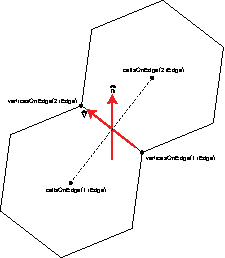
\includegraphics[height=3.5in]{shared/figures/angleEdge.pdf}
\caption{The angle of an edge refers to the angle between a vector pointing north at an edge location
and a vector pointing in the positive tangential velocity direction of the edge.}
\label{fig:angleEdge}
\end{center}
\end{figure}

The angle of each edge in an MPAS grid is provided in the variable {\it angleEdge}. The angle
given is the angle between a vector pointing north and a vector pointing in the
positive tangential direction of the edge. Referring to Fig. \ref{fig:angleEdge},
\[ {\rm angleEdge} = \arcsin\|{\bf \hat n} \times {\bf \hat v}\|, \]
where ${\bf \hat n}$ is the unit vector pointing north and ${\bf \hat v}$ is the unit vector
pointing from verticesOnEdge(1,iEdge) to verticesOnEdge(2,iEdge).

Given a wind vector $(u_\perp, u_\parallel)$ defined in term of components orthogonal to
and parallel to the edge, the earth-relative wind $(u,v)$ may be recovered as
\[
\begin{bmatrix}
u \\
v \\
\end{bmatrix}
=
\begin{bmatrix}
\cos\alpha && -\sin\alpha \\
\sin\alpha && \cos\alpha \\
\end{bmatrix}
\begin{bmatrix}
u_\perp \\
u_\parallel \\
\end{bmatrix},
\]
where $\alpha = {\rm angleEdge}$.






\end{document}

